\documentclass[10pt, compress]{beamer}
\usetheme[conference=KoM,venue=Remote, date=03/13/2017, titleprogressbar, logo=RFX-logo]{Eurof}
\usepackage{listings,amsmath,multimedia, amssymb}
\usepackage{../beamerclass/tangocolors}
\usepackage{../beamerclass/rfxcolor}
% for drawing
\usepackage{pgf}
\usepackage{tikz}
\usetikzlibrary{arrows,shapes,backgrounds}
\usepackage{../beamerclass/onimage}
\usepackage[export]{adjustbox}
\usepackage{bm}
% for font
\usepackage[absolute,overlay]{textpos}
  \setlength{\TPHorizModule}{1mm}
  \setlength{\TPVertModule}{1mm}

\usepackage[style=nature,citestyle=authoryear-comp,defernumbers=true,maxnames=2,firstinits=true,
uniquename=init,backend=bibtex8,arxiv=abs,mcite]{biblatex}
\bibliography{biblio}
\renewcommand*{\bibfont}{\footnotesize}
\renewcommand*{\citesetup}{\footnotesize}
\usepackage[export]{adjustbox}
\makeatother
\mode<presentation>
\makeatletter
% add a macro that saves its argument
\newcommand{\footlineextra}[1]{\gdef\insertfootlineextra{#1}}
\newbox\footlineextrabox
% for reducing font on a single slide
\newcommand\Fontvi{\fontsize{8}{7.2}\selectfont}
\title{Topic 21: AUG experiment}
\date{24 April 2017}
\author[Topic 21 Scientific Team]{Topic 21 Scientific Team}
\begin{document}
\tikzstyle{every picture}+=[remember picture]
\maketitle

\begin{frame}{L-Mode}
\Fontvi
  \vspace{-1cm}
\begin{columns}
  \begin{column}{0.5\textwidth}
    \centering{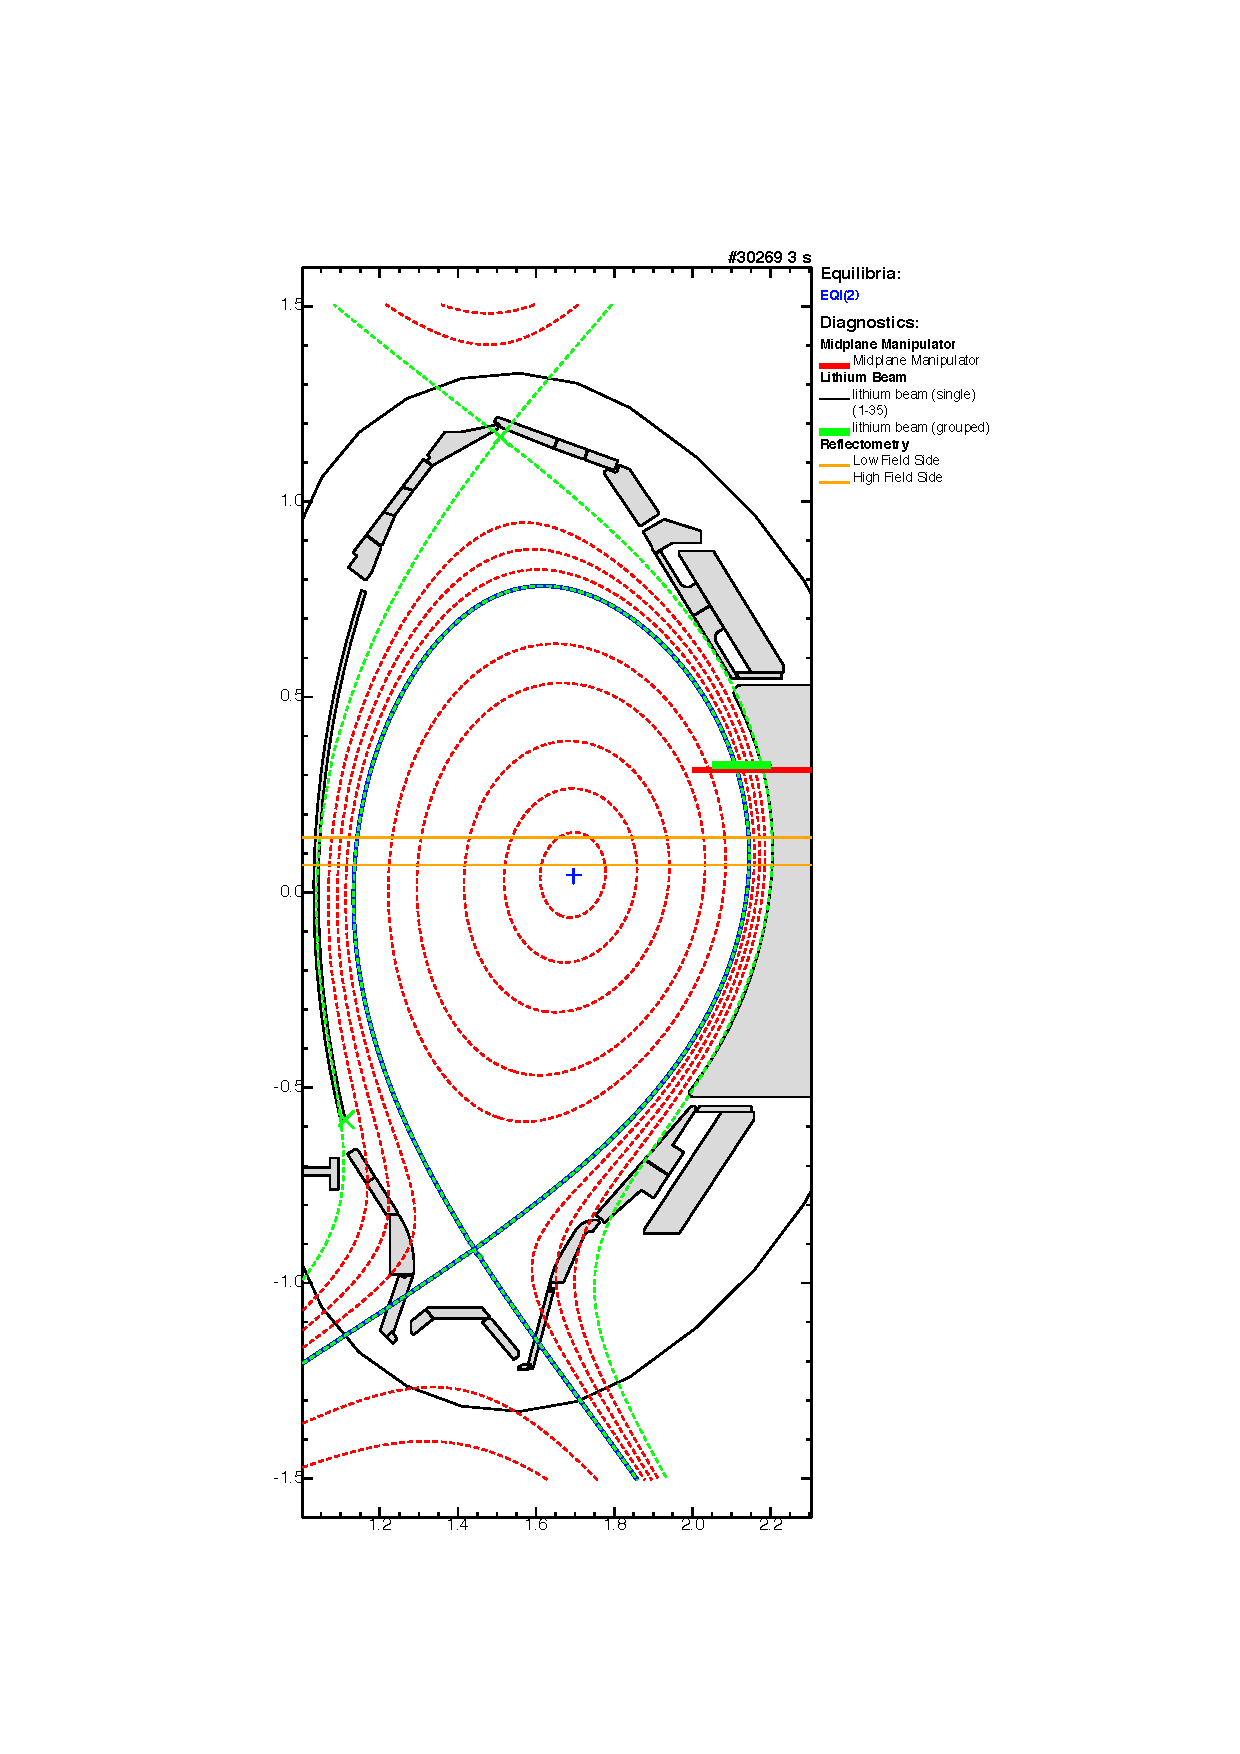
\includegraphics[height=\textheight]{pdfbox/30269Shape}}
  \end{column}
  \begin{column}{0.5\textwidth}
    \begin{description}
      \item[\# 1] \textbf{EOC} Shape, 0.8MA, B$_{\phi}$ = -2.5 T, 0.5MW NBI heating,
        fueling as reference 30269, heating starting together with
        fueling
      \item[\# 2] Same density ramp and heating with I$_p$ = 0.61 MA,
        B$_{\phi}$ = -1.9T (reduced current with the same q$_{95}$)
      \item[\# 3] Same density ramp and heating with I$_p$ = 0.99 MA,
        B$_{\phi}$ = -3.1T (increased current with the same q$_{95}$)
      \item[\# 4] Same density ramp and heating B$_{\phi}$ = -2.5T and I$_{p}$ = 0.99 MA
      \item[\# 5] Same density ramp and heating B$_{\phi}$ = -2.5T and I$_{p}$ = 0.61 MA
    \end{description}
  
  \end{column}
\end{columns}
\end{frame}

\begin{frame}{H-Mode}
\Fontvi
  \vspace{-1cm}
\begin{columns}
  \begin{column}{0.5\textwidth}
    \centering{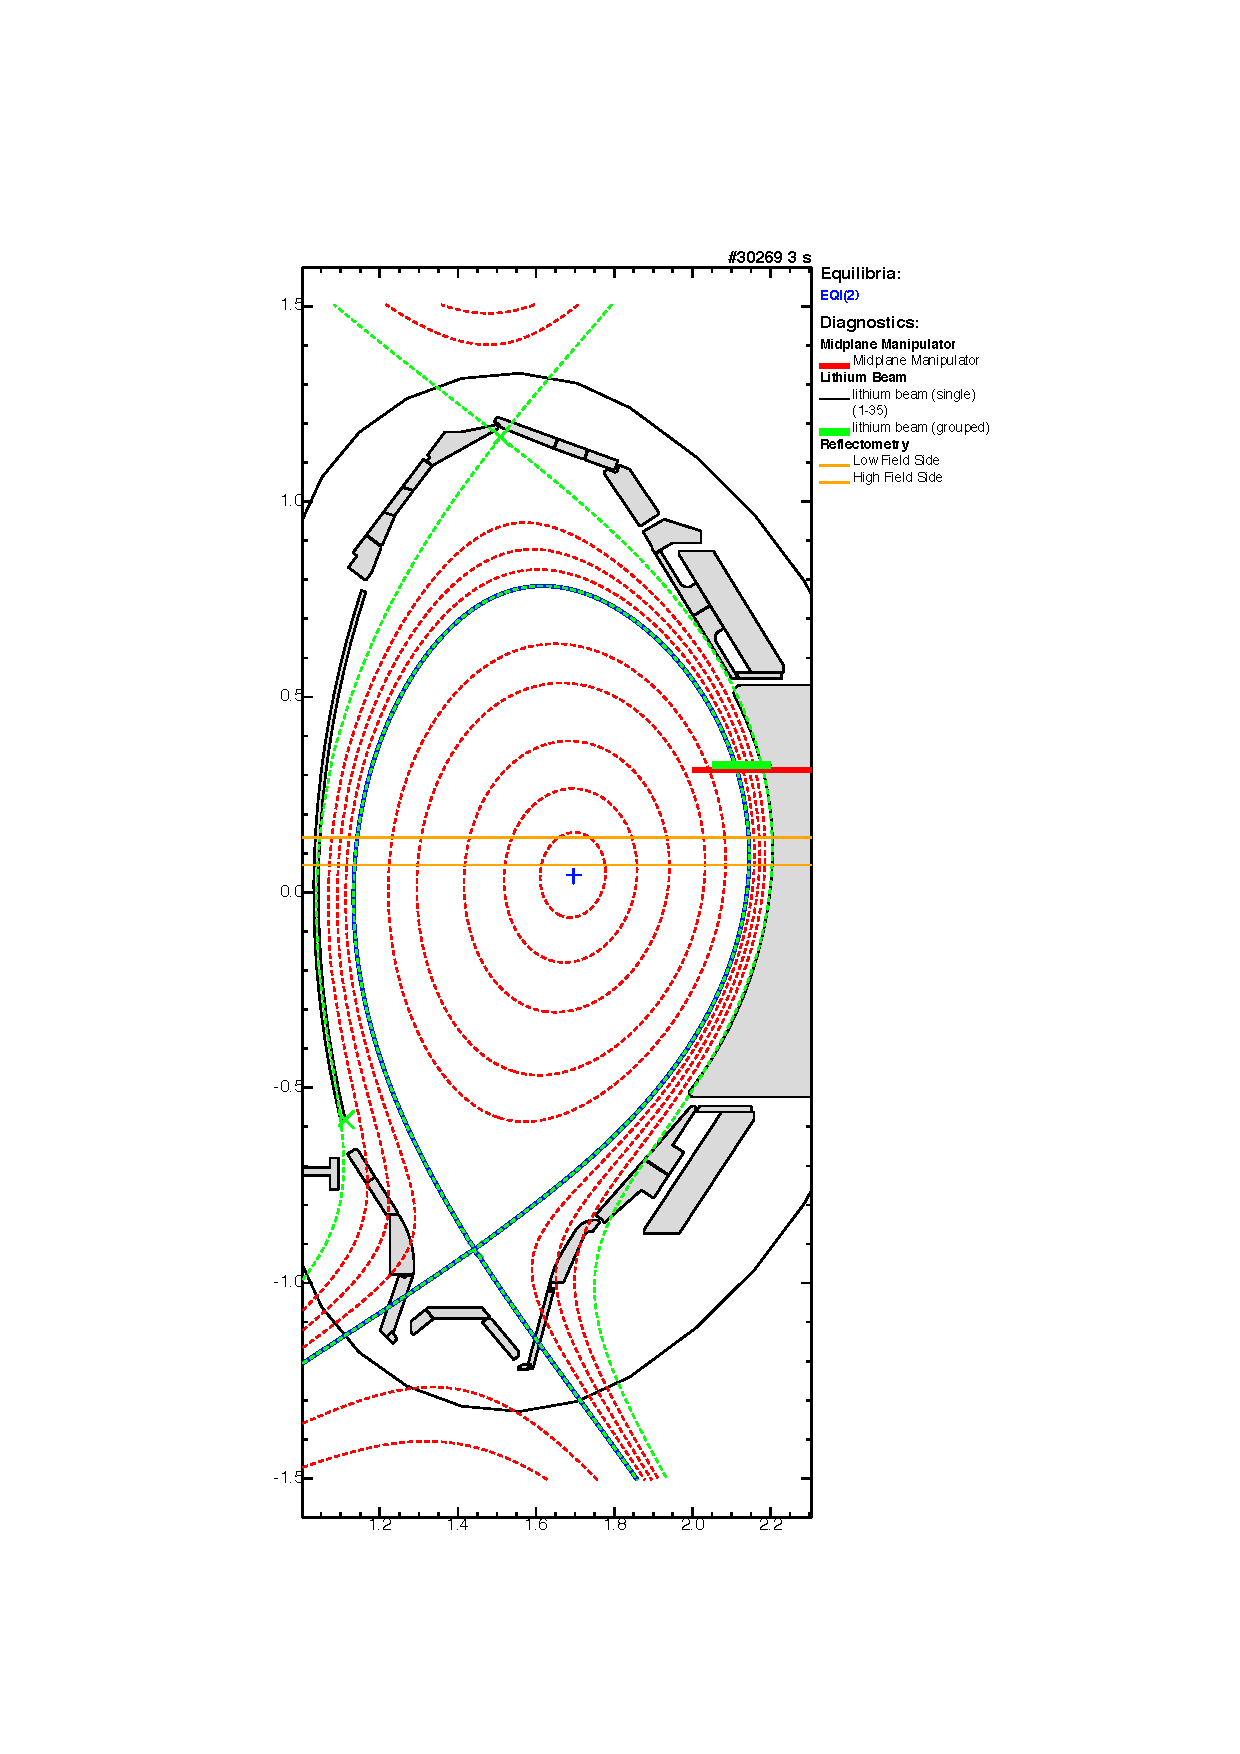
\includegraphics[height=\textheight]{pdfbox/30269Shape}}
  \end{column}
  \begin{column}{0.5\textwidth}
    \begin{description}
      \item[\# 6] \textbf{EOC} Shape, repeat \# 33478 with P$_{NBI}$ =
        4MW, D$_2$ puffing starting at 4s up to 35$\times 10^{21}$ @
        6s. 1 Plunge of probe in safe position
      \item[\# 7] Repeat 6 adding N in feed-forward. Keep similar
        value as reference (since we are already increasing the fueling)
    \end{description}
  \end{column}
\end{columns}
\end{frame}


\begin{frame}{Required diagnostic and analysis}
  \begin{itemize}
    \item[$\boxtimes$] Midplane Manipulator
    \item[$\boxtimes$] Li-Beam profiles (inter-ELMs one in the H-Mode
      shots) and fluctuations
    \item[$\boxtimes$] RFA \#2
    \item[$\boxtimes$] Divertor probes. Evaluation inter-shot of
      profiles and rollover density. Divertor collisionality
    \item[$\boxtimes$] Neutral profiles
    \item[$\square$] Infrared for probe head monitoring
    \item[$\boxtimes$] Reflectometer including the multi-channel one
      for the operation at 1.9 T
    \item[$\square$] Bolometer/AXUV in the divertor region. We need
      the monitoring of radiation front movement. Can we get inverted
      and tomography inter shot?
    \item[$\square$] Gauges and neutral measurement
    \item[$\boxtimes$] SXR 
    \end{itemize}
\end{frame}

\begin{frame}{HFF probe head}
  \begin{columns}
    \begin{column}{0.5\textwidth}
      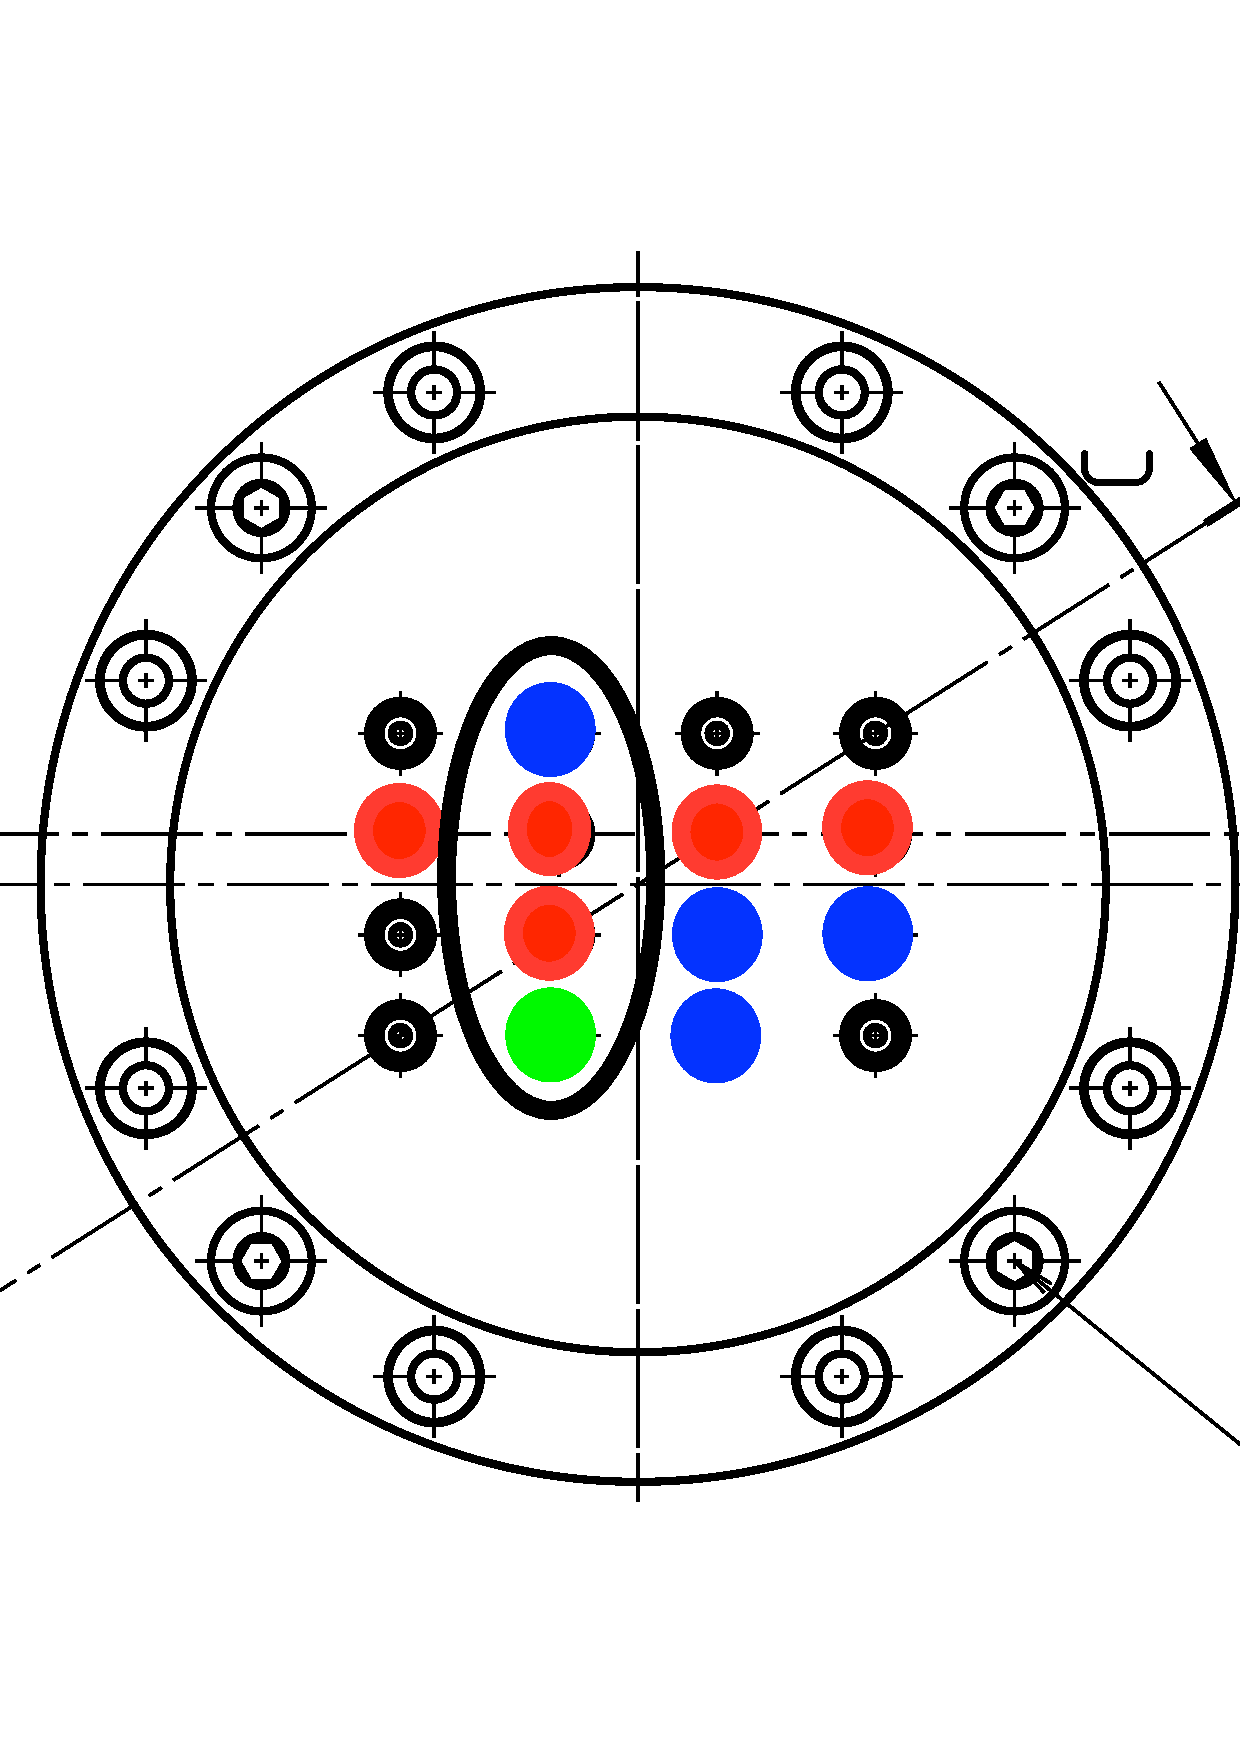
\includegraphics[width=.9\textwidth, angle=-10]{pdfbox/HeadConfiguration}
    \end{column}
    \begin{column}{0.5\textwidth}
      \begin{itemize}
      \item \textcolor{red}{Ion saturation current}
      \item \textcolor{blue}{Floating potential}
        \item \textcolor{green}{Swept probe for T$_e$ and $n_e$}
        \item Intershot analysis for blob-size, autocorrelation
      \end{itemize}
    \end{column}
  \end{columns}
  
\end{frame}
\end{document}

